\documentclass[10pt,twoside]{article}

% !TEX program = pdflatex
% ==================== NeurIPS 样式（投稿稿式）====================
\usepackage[preprint]{neurips_2025}
\geometry{marginparwidth=0.4in, marginparsep=0.1in}

% ==================== 数学与符号 ====================
\usepackage{amsmath,amssymb,amsfonts,amsthm}
\usepackage{mathtools}
\usepackage{bm}
\usepackage{siunitx}

% ==================== 图表 ====================
\usepackage{graphicx}
\usepackage{xcolor}
\usepackage{booktabs}
\usepackage{multirow}
\usepackage{array}
\usepackage{tikz}
\usetikzlibrary{arrows.meta,positioning,calc,fit,shapes.geometric}
\usepackage{caption}
\usepackage{subcaption}

% ==================== 浮标布局 ====================
\usepackage[section]{placeins}          % 浮标不得跨节漂移
\renewcommand{\topfraction}{0.92}
\renewcommand{\bottomfraction}{0.85}
\renewcommand{\textfraction}{0.06}
\renewcommand{\floatpagefraction}{0.72}

% ==================== 链接与引用 ====================
\usepackage[colorlinks=true, linkcolor=black, citecolor=black, urlcolor=black]{hyperref}
\usepackage{url}
\usepackage{enumitem}

% ==================== 自定义命令 ====================
\newcommand{\stopgrad}{\operatorname{sg}}
\newcommand{\topk}{\operatorname{TopK}}
\newcommand{\softmax}{\operatorname{softmax}}
\newcommand{\softplus}{\operatorname{softplus}}
\newcommand{\sigmoid}{\operatorname{sigmoid}}
\newcommand{\R}{\mathbb{R}}
\newcommand{\E}{\mathbb{E}}

% ==================== 定理环境 ====================
\theoremstyle{definition}
\newtheorem{definition}{Definition}[section]
\newtheorem{assumption}{Assumption}[section]
\theoremstyle{plain}
\newtheorem{theorem}{Theorem}[section]
\newtheorem{lemma}{Lemma}[section]
\newtheorem{corollary}{Corollary}[section]
\newtheorem{proposition}{Proposition}[section]
\theoremstyle{remark}
\newtheorem{remark}{Remark}[section]

% ==================== 元信息 ====================
\title{Reconstructing Frozen Heterogeneous Pretrained Models:\\
Sublayer Fusion, Coordinated Routing, and Chimera Distillation}

\author{
    Anonymous Author(s)\\
    Affiliation\\
    \texttt{email@example.com}
}

\begin{document}

\maketitle

\begin{abstract}
Combining heterogeneous pretrained models---bidirectional encoders, causal decoders, and vision transformers that differ in architecture, hidden width, and modality---usually requires joint retraining, architecture surgery, or lossy output-level ensembling. We study how such models can be \emph{reconstructed} while every base stays frozen, in three steps. \textbf{(i) Sublayer fusion.} A shared sparse Top-$K$ router selects one of $M$ frozen architectural experts per token; semantic aligners map mismatched hidden spaces into one shared routing space; experts are fused residually with per-expert gates. Across four aligner designs we measure a strict but \emph{saturating} ladder (linear $<$ mean $<$ cross-architecture attention $<$ mixture), and a capacity-matched control shows the ceiling is a matter of design rather than of parameter count. \textbf{(ii) Coordinated routing.} We ask how a global hub should influence the shared router, and prove that modulating the softmax temperature (gate-style) is the only one of four hub modes satisfying perfect degeneration, order preservation, boundedness, and low overhead at once; we also diagnose a hidden failure mode in which tanh saturation severs the gradient to the hub during long training. \textbf{(iii) Independent-model reconstruction.} Chimera distillation collapses the ensemble into a single-base student, and a weight scan over the loss shows that the apparent ``student beats teacher'' margin is entirely attributable to a direct-target term rather than to concept-direction transfer or variance averaging. Because fused inference keeps every base alive and distillation is a deployment device, the study is only as trustworthy as its evaluation. We therefore apply a uniform \emph{out-of-sample discipline} across the whole stack, and it overturns several of our own in-sample findings: the in-sample best hub mode is not the out-of-sample best, an advertised corpus-scale boundary is not established, and long-training and repair gains shrink to noise. What survives held-out evaluation is the alignment-ladder ceiling, the attention-path advantage, and the scale-heterogeneous fusion gain (\S\ref{sec:scale-hetero-exp}), whose in-sample margin of $+26.7\%$ is retained out of sample. We report the negative results that bound the method---component composition, nested aligners, multi-teacher distillation, and toy multimodal benchmarks---from hundreds of seeded end-to-end runs across 41 versioned engineering generations and 430 unit and integration tests.
\end{abstract}

\section{Introduction}
\label{sec:intro}

Practitioners rarely have the luxury of one perfect pretrained model. A working pipeline may need a bidirectional encoder for text understanding, a causal decoder for generation, and a vision transformer for perception. Three ways to combine such models dominate current practice, and each is unsatisfying. Joint multi-task retraining is expensive and re-opens the pretraining budget. Output-level ensembling keeps every model alive at inference and blends predictions that were never trained to complement each other. Weight merging \citep{ilharco2023,yadav2023,wortsman2022} requires the merged models to share architecture and initialization, which rules out heterogeneous bases outright.

This paper studies a fourth option, one level lower, and asks how far it can be pushed. Within a transformer block, the feed-forward (FFN) sublayer is the most modular and the most replaceable component: it acts position-wise, it carries a large share of the parameters, and its role as a key--value memory \citep{geva2021} suggests that \emph{which} memory bank is consulted can be decided per token. We therefore treat frozen heterogeneous bases as a resource to be \emph{reconstructed} in three stages, each of which removes one of the three obstacles above.

\textbf{Stage 1 --- sublayer fusion.} We rebuild the FFN sublayer itself as a \textbf{heterogeneous micro-fusion layer}: a shared, sparse Top-$K$ router selects among $M$ frozen architectural experts; rectangular projections or learned semantic aligners map mismatched hidden spaces ($D_m \in \{192, 312, 768\}$) into one shared routing space; per-expert gates, channel-wise alignment, and INT4 pseudo-quantization noise complete the layer. No base model is modified, and only alignment, routing, and gate parameters are trained. A dual-path extension makes the attention sublayers routable as well, so that a token can independently select one attention expert and one FFN expert.

\textbf{Stage 2 --- coordinated routing.} Fusion imposes a new question that within-architecture MoE never faces: the experts disagree about \emph{what a good routing decision is}, because they were never trained together. Should a global hub---a shared vector summarizing the ensemble---influence the router, and if so, how? We formalize five design constraints and prove that among four candidate hub mechanisms, only temperature modulation (gate-style coordination) satisfies all five: it degenerates exactly to the no-hub baseline when disabled, preserves logit ordering by construction, is bounded, and costs $O(D_{\text{shared}})$ parameters. We also identify a hidden failure mode---tanh saturation in the temperature scalar severs the gradient to the hub under long training---and two repairs that restore gradient flow.

\textbf{Stage 3 --- independent-model reconstruction.} Fusion has a deployment cost: the fused system still needs every base alive at inference. We close the loop with \textbf{chimera distillation}, in which a single-base student---a real frozen TinyBERT \citep{jiao2020} with a low-rank adapter \citep{hu2022}---is trained to reproduce the fused teacher's output from its \emph{own} modality's input alone.

\textbf{The thread that holds the three stages together.} Each stage is a claim about a quantity measured at small scale, and each claim is only as good as its evaluation. We therefore adopt a single discipline throughout: every headline number is validated on inputs the model never trained on. This discipline is not cosmetic. Applying it retroactively to our own earlier results changed several of them, in both directions. On the negative side, the in-sample best hub mode is not the best out-of-sample, an advertised corpus-scale boundary does not survive, and the two gradient repairs turn out not to move fusion MSE at all. On the positive side, the alignment-ladder ceiling, the attention-path advantage, and the scale-heterogeneous fusion gain (\S\ref{sec:scale-hetero-exp}) all survive held-out evaluation intact, the last retaining $99$--$100\%$ of its in-sample margin under both a re-sampled-noise and a shifted-stimulus protocol. We report both outcomes, because a mechanism-level study whose positive results are not separated from its evaluation artifacts is not evidence.

We make the following contributions, ordered from mechanism to evidence.

\begin{enumerate}[leftmargin=1.5em, itemsep=1pt]
    \item \textbf{An alignment ladder with a measured ceiling} (\S\ref{sec:align-exp}). Replacing the frozen linear projection with a cross-base mean, then shared-key/value attention, then a mixture-of-experts aligner yields a strict ladder ($1.14 \rightarrow 0.48 \rightarrow 0.34 \rightarrow 0.26$ MSE); nesting the mixture regresses by $4.7\%$. A capacity-matched control in which the mixture aligner is reduced to bit-for-bit the attention aligner's parameter count still leaves the mixture ahead by $36.5\%$ on held-out data, so the ceiling is design, not scale.
    \item \textbf{Fusion that beats its parts, with the gain located} (\S\ref{sec:fusion-exp}). FFN-only routing beats the best single expert by $20.3\%$ and equal-weight averaging by $17.3\%$; dual-path routing raises the margin over averaging to $84.8\%$. A path decomposition shows the cross-architecture gain concentrates in the attention path---a claim that survives held-out evaluation ($+82.7\%$ in-sample, $+70.6\%$ held-out).
    \item \textbf{A uniqueness theory for routing coordination} (\S\ref{sec:hub}). Four hub modes are compared against five design constraints; gate-style temperature modulation is the only mode satisfying all five, with perfect degeneration and order preservation proved constructively (hence unfalsifiable by data leakage). We also diagnose the tanh-saturation failure mode (\S\ref{sec:diagnosis}).
    \item \textbf{An honest decomposition of chimera distillation} (\S\ref{sec:distill-exp}). A single-base student is \emph{not} shown to internalize the teacher's concept directions: a $\beta$ scan over the direct-target weight, a variance-boundedness test, and a representation-transfer probe jointly show that the entire measured margin is attributable to the direct-target term in the loss.
    \item \textbf{Out-of-sample discipline as a result in its own right} (\S\ref{sec:oos}). Across the stack we find that in-sample composition rankings are training-fit orderings, not capability rankings: the same four hub modes that rank gate first in-sample rank router-norm first out-of-sample, and the corpus-scale boundary that appears in-sample is absent out-of-sample.
\end{enumerate}

Just as informative are the boundaries. Five distinct negative results bound the method. (i)~Composing a repaired router with a stronger aligner adds nothing once the aligner already contains the repair ($+71.0\%$ vs.\ $+72.6\%$ over their common baseline). (ii)~Harder toy VQA benchmarks do not rescue multimodal evaluation---all models drop to random accuracy. (iii)~Multi-teacher distillation regresses in every configuration, and a dispatch-style reformulation removes the harm without producing any gain. (iv)~Nesting the mixture aligner with itself regresses by $4.7\%$ MSE. (v)~Pure distillation does not outperform the teacher, so the entire student-vs-teacher margin is target leakage. The recurring lesson is that adding machinery is not the same as adding capability, and measuring in-sample is not the same as measuring capability.

\section{Related Work}
\label{sec:related}

\textbf{Mixture-of-experts routing.} Conditional computation routes each input to a subset of experts \citep{jacobs1991,shazeerOutrageouslyLargeNeural2017}, and modern sparse MoE stacks scale this to trillion-parameter regimes \citep{fedus2022,zoph2022}. Mixtral 8x7B \citep{jiang2024mixtral} delivers 47B total / 13B active parameters per token via top-2 token-level routing over eight FFN copies, with measured temporal locality and clear domain specialization. Soft routing addresses MoE instability and load imbalance through slot-based differentiable mixtures \citep{puigcerver2024softmoe}, and fine-grained expert segmentation with shared-expert isolation \citep{dai2024}, together with branch-and-train-then-mix recipes \citep{sukhbaatar2024btx}, refines specialization further. In all of these systems the experts are \emph{homogeneous}: they share architecture, dimension, and training. Sparse upcycling \citep{komatsuzaki2023} converts a dense checkpoint into an MoE by cloning and perturbing its FFNs, again producing homogeneous experts. Our experts are the opposite: entire pretrained models with different architectures, tokenizers, and modalities, kept frozen. The routing problem correspondingly changes from balancing identical experts to aligning incompatible representation spaces---which is the subject of \S\ref{sec:layer} and \S\ref{sec:hub}.

\textbf{Heterogeneous foundation-model collaboration.} A growing line of work studies collaboration between pretrained models that do \emph{not} share architecture. Within the homogeneous limit, Symphony-MoE \citep{wang2025symphony} upcycles several like-architected but differently-pretrained LLMs by harmonizing shared backbones via SLERP and re-permuting FFN neurons through a linear assignment problem. The harder cross-architecture case is studied under cross-architecture distillation \citep{wang2024scalekd}, whose cross-attention projector plus dual-view mimicking is the closest published antecedent to our fusion layer. For orchestrated heterogeneous LLM inference in cross-border e-commerce relevance, \citet{liu2026orchestrating} show that \emph{concatenating} expert embeddings beats weighted averaging for models with distinct embedding manifolds---a geometric argument our four-mode comparison corroborates from the opposite direction (the modes that preserve per-expert information beat the one that averages it). Expert-aware post-training quantization \citep{du2026eaquant} validates the cross-expert channel-similarity assumption that underpins our channel alignment. Together these works delineate a \emph{heterogeneity spectrum} (Figure~\ref{fig:het-spectrum}) within which we sit at the hardest corner: same architecture, same modality, and same manifold is the easy limit; our setting is simultaneously different on all three axes.

\begin{figure}[htbp]
\centering
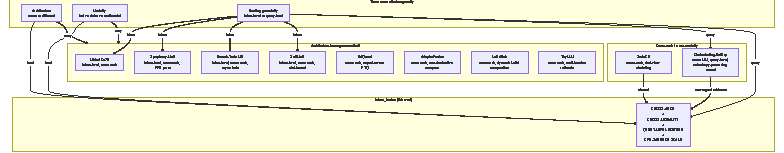
\includegraphics[width=0.95\textwidth]{figs/mermaid/heterogeneity_spectrum.pdf}
\caption{\textbf{Heterogeneity spectrum} of recent foundation-model collaboration work across three axes: \emph{architecture} (same vs different), \emph{modality} (text / vision / multimodal), and \emph{routing granularity} (token-level vs query-level). Existing work populates the architecture-homogeneous limit; the architecture-heterogeneous limit is sparsely populated, with ScaleKD and Orchestrating-HetExp as the closest antecedents. This paper sits at the intersection of all three harder axes simultaneously, on CPU-sandbox scale rather than industrial.}
\label{fig:het-spectrum}
\end{figure}

\textbf{Model merging and upcycling.} Task arithmetic \citep{ilharco2023}, TIES-merging \citep{yadav2023}, and model soups \citep{wortsman2022} combine \emph{weights} of models that share a backbone. Heterogeneous bases cannot be merged this way; our fusion layer is the corresponding mechanism for the heterogeneous case, operating through activations instead of parameter addition.

\textbf{Parameter-efficient adaptation.} Adapters \citep{houlsby2019} and LoRA \citep{hu2022} freeze a base and train small insertions. We use the same philosophy, but the frozen part is a \emph{pool} of heterogeneous bases and the trained part is the inter-base machinery (projections, aligners, router, gates). AdapterFusion \citep{pfeiffer2021} composes per-task adapters non-destructively through a learned attention combiner, and \citet{huang2024lorahub} generalize this to a dynamic linear combination of per-task LoRA modules optimized by black-box search---both demonstrate the non-destructive composition principle we independently adopt for cross-architecture fusion. Our aligner ladder can be read as an activation-level analogue, and our multi-teacher negative result (\S\ref{sec:distill-exp}) echoes Pfeiffer et al.'s finding that naive source combination is not free.

\textbf{Knowledge distillation.} Distillation transfers a teacher's behavior to a smaller student \citep{hintonDistillingKnowledgeNeural2015,sanh2019,gou2021}; multi-teacher variants are known \citep{you2017}, and recent multi-teacher LLM distillation uses rationale-augmented objectives to recover knowledge diversity \citep{tian2025tinyllm}. Chimera distillation differs in both directions: the teacher is a multi-base \emph{ensemble}---echoing the collective-intelligence framing of mixture-of-agents \citep{wang2024moa} and the stacked-generalization idea \citep{wolpertStackedGeneralization1992}, though our collaboration operates at the representation level through learned routing rather than at the output level---and the student sees only one base's input yet must reproduce the ensemble's fused output. Quantization-aware training injects fake-quantization noise during training \citep{dettmers2022}; we use INT4 fake quantization on expert outputs as regularization and hardware-realism pressure, not as a deployment compression claim. Teacher-assistant distillation \citep{mirzadeh2020} is the nearest analogue of the effect we decompose in \S\ref{sec:distill-exp}: an intermediate or cleaner target helps the student, and here the ``cleaner target'' is partly the direct-target term, which we show to be the whole story.

\textbf{Global coordination of selection.} The question of stage 2---whether a global signal should coordinate a selection mechanism---has a long history. Global Workspace Theory \citep{baarsCognitiveTheoryConsciousness1988} motivates a broadcast-style hub, but we treat it as design inspiration rather than as a testable prediction, since it does not by itself specify the functional form of the interaction. Sparse-gated MoE \citep{shazeerOutrageouslyLargeNeural2017} and Linformer-style global mixing \citep{wangLinformerSelfAttentionLinear2020} are the closest architectural relatives. Global mixers of the linear-attention and state-space family \citep{katharopoulos2020,gu2022s4,gu2023mamba} sit on an orthogonal axis: they mix across \emph{sequence positions} within one model by carrying content in a state, whereas our hub coordinates across the \emph{expert} axis of many frozen models at one position by modulating routing \emph{certainty}---a scalar temperature that rescales logits without adding content, preserving logit ordering by construction and degenerating exactly when disabled. Content-carrying states satisfy neither property in general, so the two mechanisms are composable rather than competing.

\section{Method I: Heterogeneous sublayer fusion}
\label{sec:method}

\subsection{Problem setup}
\label{sec:setup}

Let $\mathcal{B} = \{B_1, \dots, B_M\}$ be $M$ frozen pretrained bases with hidden sizes $D_m$ and, in general, different architectures: a bidirectional encoder (TinyBERT, $D{=}312$) \citep{jiao2020,devlin2019}, a causal decoder (TinyLlama-110M, $D{=}768$), and a vision transformer (ViT-tiny, $D{=}192$) \citep{dosovitskiy2021}. Each base consumes its own tokenizer or processor and produces hidden states $h_m \in \R^{S \times D_m}$ natively; we never force a shared encoder. The goal is a fusion layer operating in a shared space of width $D_{\text{shared}} = 256$ such that (i) every base remains frozen, (ii) only alignment, routing, and gate parameters are trained, and (iii) the layer degrades gracefully---disabling any single expert leaves a working system.

\subsection{The heterogeneous fusion layer}
\label{sec:layer}

\begin{figure}[htbp]
\centering
\resizebox{\textwidth}{!}{%
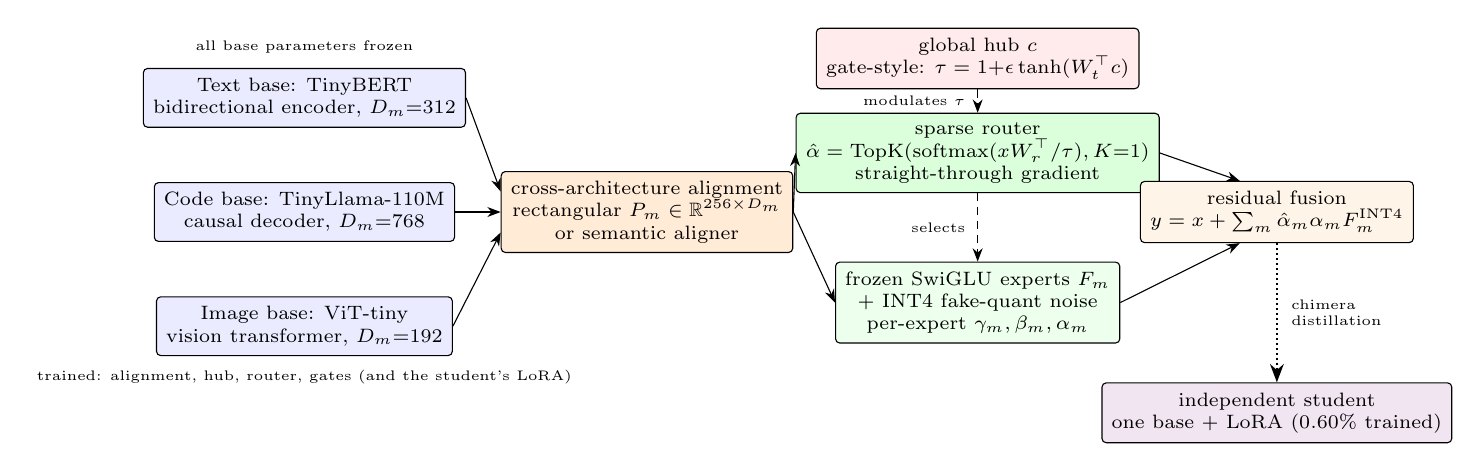
\begin{tikzpicture}[
  font=\scriptsize, >=Stealth, node distance=3mm,
  base/.style={draw, rounded corners=1.5pt, align=center, inner sep=3.5pt, fill=blue!8, minimum width=34mm},
  stage/.style={draw, rounded corners=1.5pt, align=center, inner sep=3.5pt},
  aligner/.style={stage, fill=orange!16},
  router/.style={stage, fill=green!14},
  expert/.style={stage, fill=green!7},
  hub/.style={stage, fill=red!8},
  fuse/.style={stage, fill=orange!9},
  student/.style={stage, fill=violet!10},
  lbl/.style={font=\tiny, align=center},
]
\node[base] (bert) at (0, 1.45) {Text base: TinyBERT\\ bidirectional encoder, $D_m{=}312$};
\node[base] (llama) at (0, 0) {Code base: TinyLlama-110M\\ causal decoder, $D_m{=}768$};
\node[base] (vit) at (0, -1.45) {Image base: ViT-tiny\\ vision transformer, $D_m{=}192$};
\node[lbl, above=0.6mm of bert] {all base parameters frozen};
\node[lbl, below=0.6mm of vit] {trained: alignment, hub, router, gates (and the student's LoRA)};

\node[aligner] (alg) at (4.35, 0) {cross-architecture alignment\\ rectangular $P_m \in \R^{256 \times D_m}$\\ or semantic aligner};

\node[hub] (hub) at (8.55, 1.95) {global hub $c$\\ gate-style: $\tau = 1{+}\epsilon\tanh(W_t^\top c)$};
\node[router] (rout) at (8.55, 0.75) {sparse router\\ $\hat\alpha = \topk(\softmax(x W_r^\top/\tau), K{=}1)$\\ straight-through gradient};
\node[expert] (exp) at (8.55, -1.15) {frozen SwiGLU experts $F_m$\\ + INT4 fake-quant noise\\ per-expert $\gamma_m, \beta_m, \alpha_m$};

\node[fuse] (fu) at (12.35, 0) {residual fusion\\ $y = x + \sum_m \hat\alpha_m \alpha_m F_m^{\text{INT4}}$};

\node[student] (stu) at (12.35, -2.55) {independent student\\ one base $+$ LoRA ($0.60\%$ trained)};
\draw[->, densely dotted, thick] (fu.south) -- node[lbl, right=1.5pt, align=left] {chimera\\ distillation} (stu.north);

\draw[->] (bert.east) -- ($(alg.west)!0.5!(alg.north west)$);
\draw[->] (llama.east) -- (alg.west);
\draw[->] (vit.east) -- ($(alg.west)!0.5!(alg.south west)$);
\draw[->] (alg.east) -- (rout.west);
\draw[->] (alg.east) -- (exp.west);
\draw[->, densely dashed] (hub.south) -- node[lbl, left=1pt] {modulates $\tau$} (rout.north);
\draw[->, densely dashed] (rout.south) -- node[lbl, left=1pt] {selects} (exp.north);
\draw[->] (rout.east) -- (fu.140);
\draw[->] (exp.east) -- (fu.220);
\end{tikzpicture}}%
\caption{Heterogeneous micro-fusion, coordinated routing, and chimera distillation. Three frozen pretrained bases with different architectures and hidden widths are natively encoded, aligned into a shared 256-dimensional space, and sparsely routed ($K{=}1$) to frozen SwiGLU experts whose outputs carry INT4 fake-quantization noise. A global hub modulates the softmax temperature of the shared router (\S\ref{sec:hub}). Chimera distillation then collapses the ensemble into one independent single-base student (\S\ref{sec:distill}).}
\label{fig:overview}
\end{figure}

Figure~\ref{fig:overview} shows the layer. Given the residual-stream input $x \in \R^{B \times S \times D_{\text{shared}}}$, each expert $m$ computes
\begin{align}
\label{eq:expert}
h_m &= \stopgrad(x) \odot \gamma_m + \beta_m, \qquad
\tilde F_m = Q_{\text{INT4}}\big(F_m(h_m)\big), \\
F_m(h) &= \big(\mathrm{SiLU}(h W^{\text{gate}}_m) \odot (h W^{\text{up}}_m)\big)\, W^{\text{down}}_m,
\end{align}
where $Q_{\text{INT4}}$ is group-wise (group size 128) 4-bit fake quantization with a straight-through estimator in the backward pass. Three deliberate choices shape the layer.

\textbf{Gradient truncation.} The expert input is detached ($\stopgrad$), so the frozen bases' intermediate activations never enter the autograd graph. Activation memory drops from $O(M L D_{\text{ff}})$ to $O(L D_{\text{shared}})$ plus adapter parameters, which is what makes $M$-base fusion trainable on CPU at all. The cost is that experts cannot shape upstream representations through gradients; the router and gates carry all adaptation.

\textbf{Sparse routing with straight-through gradients.} The router computes logits $z = x W_r^\top$ from the \emph{clean} pre-noise input, $\alpha = \softmax(z/\tau)$, and the hard selection $\hat\alpha = \topk(\alpha, K)$ ($K{=}1$ unless stated) is applied in the forward pass while the backward pass follows the softmax weights, in the spirit of straight-through estimators \citep{bengio2013}. Routing on the clean input keeps router decisions from chasing the quantization noise it would otherwise induce. The temperature $\tau$ is the hub's sole channel of influence and is $1$ unless a hub is fitted (\S\ref{sec:hub}).

\textbf{Residual fusion with positive gates.} The layer output is
\begin{equation}
\label{eq:fuse}
y = x + \sum_{m=1}^{M} \hat\alpha_m \, \alpha_m \, \tilde F_m(h_m),
\end{equation}
with $\alpha_m \sim \mathcal{U}(0.01, 0.1)$ at initialization. The positive, non-trivial initialization avoids the near-zero-gate dead lock: gates initialized at $10^{-4}$ scale receive gradients too small to escape, which we observed as flat training curves before adopting the uniform initialization.

\subsection{Two-phase training protocol}
\label{sec:training}

Routing is fragile early in training---random router weights produce noise selections that poison the expert gates. Training therefore runs in two phases. \textbf{Phase 1} (first $10\%$ of steps): routing is forced uniform ($\hat\alpha_m = 1/M$, detached) and the router is frozen, so only alignment and gate parameters learn. \textbf{Phase 2} (remaining $90\%$): the router unlocks and Top-$K$ selection activates, with the loss
\begin{equation}
\label{eq:loss}
\mathcal{L} = \mathcal{L}_{\text{task}} + \lambda_1 \mathcal{L}_{\text{balance}} + \lambda_2 \mathcal{L}_{z},
\end{equation}
where $\mathcal{L}_{\text{balance}}$ encourages even expert load and $\mathcal{L}_{z}$ regularizes router logits. Optimizer groups isolate learning rates: $10^{-4}$ for the router and hub, $10^{-2}$ for alignment parameters, and $10^{-3}$ for the output gates $\alpha_m$. The router must move slowly because its selections are discrete; the alignment layers can move quickly because their gradients are dense.

\subsection{The alignment ladder}
\label{sec:align}

The shared space is where heterogeneous bases meet, and how it is constructed turned out to matter more than anything else in the stack. We evaluate four designs of increasing sophistication (Figure~\ref{fig:ladder-chain}):

\begin{description}[leftmargin=1.4em, itemsep=1pt]
    \item[Linear projection (baseline).] Each base's hidden state passes through a rectangular projection $P_m \in \R^{D_{\text{shared}} \times D_m}$, orthogonal-initialized and frozen. Bases are projected independently and know nothing about each other.
    \item[Mean aligner.] Learned per-base down-projections $W_m \in \R^{d \times D_m}$ followed by a cross-base mean of the projected representations.
    \item[Cross-architecture attention aligner.] Each base is projected to the shared width; the cross-base mean provides shared keys and values; each base queries the shared context with its own query projection---the standard query/key/value separation of cross-attention \citep{vaswani2017}---and adds the attended concept vector residually. Every base therefore reads a concept summary written by \emph{all} bases.
    \item[Mixture aligner.] Each base contributes $n{=}4$ small shared experts (two-layer MLPs) to a pooled bank of $M \times n$ experts. Expert outputs serve as queries against a shared key/value context derived from their mean, and the attended outputs are aggregated. The aligner itself becomes a tiny mixture-of-experts over the heterogeneous sources.
\end{description}

\begin{figure}[htbp]
\centering
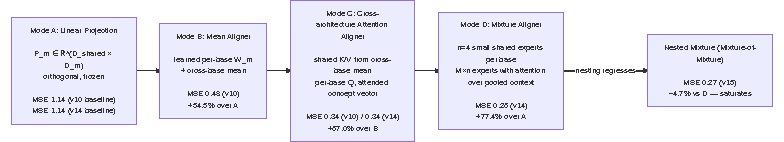
\includegraphics[width=0.95\textwidth]{figs/mermaid/alignment_ladder.pdf}
\caption{\textbf{The alignment ladder} as a strict-but-saturating chain: mode A (linear projection) $\rightarrow$ B (mean aligner) $\rightarrow$ C (cross-architecture attention) $\rightarrow$ D (mixture-of-experts aligner). Each mode improves on the previous one in 5-seed MSE; nesting the mixture regresses by $4.7\%$ (\S\ref{sec:align-exp}), marking the ceiling.}
\label{fig:ladder-chain}
\end{figure}

Two empirical facts motivate the ladder. First, \emph{native encoding is not optional}: in an early control where all three modalities were tokenized and encoded by the same BERT, the fusion gain over a single expert collapsed from $+20.3\%$ to $+4.0\%$. Uniform encoding erases exactly the architectural differences the router is supposed to exploit. Second, the ladder is \emph{strict but saturating}: each mode improves on the previous one, and the improvement stops at the mixture aligner (\S\ref{sec:align-exp})---a ceiling we hold as a scale-bounded hypothesis, not a law.

\subsection{Dual-path routing: making attention routable}
\label{sec:dualpath}

The FFN-only layer routes among memory banks but always consumes the same attention output. The dual-path extension makes the attention sublayers routable too: each token independently selects one \emph{attention expert} and one \emph{FFN expert}, from two pools that may come from different bases. Attention experts expose the native Q/K/V/O projections of the base's first block; the selected expert's attention is recomputed in its native space and projected back through $P_m$. Per-expert optimizer groups implement the learning-rate isolation of \S\ref{sec:training} per expert. The dual-path design asks whether cross-architecture complementarity lives in the FFN weights, in the attention patterns, or in both---and the path decomposition in \S\ref{sec:fusion-exp} gives a sharp answer.

\section{Method II: Coordinating the shared router}
\label{sec:hub}

\subsection{Four hub modes}
\label{sec:modes}

Heterogeneous experts were never trained together and disagree about what a good routing decision is. A natural response is a \emph{global hub}: a shared vector $c \in \R^{D_{\text{shared}}}$ that summarizes the ensemble and influences the router. We consider four ways the hub can act on the routing logits $z_m$:

\begin{definition}[Broadcast mode]
$z_m^{(\text{bc})} = z_m + (U c)_m$, where $U \in \R^{M \times D_{\text{shared}}}$ is learnable. The hub adds a bias to each expert's logit.
\end{definition}

\begin{definition}[Router-norm mode]
$z_m^{(\text{rn})} = \mathrm{LayerNorm}(z_m + U c)$. Broadcast, then normalize.
\end{definition}

\begin{definition}[Adaptive-EMA mode]
$\text{decay} = \sigmoid(\alpha \cdot \|c\|)$. The hub controls its own exponential-moving-average decay rate; the EMA state then enters the logits.
\end{definition}

\begin{definition}[Gate-style mode (proposed)]
$t_{\text{scalar}} = W_t^\top c$, $\tau = 1 + \epsilon \cdot \tanh(t_{\text{scalar}})$, $z_m^{(\text{g})} = z_m / \tau$. The hub modulates the softmax temperature.
\end{definition}

The modes differ in \emph{how} the hub enters the decision. Broadcast and router-norm \emph{add} a hub-dependent term to the logits; adaptive-EMA lets the hub shape an accumulating state; only gate-style \emph{scales} the logits by a positive scalar. That structural difference is what the next subsection turns into a theorem.

\subsection{Design constraints and why only gate-style satisfies them}
\label{sec:theory}

We formalize five constraints that any hub mechanism for a frozen-expert router should satisfy:
\begin{itemize}[leftmargin=1.5em, itemsep=1pt]
    \item \textbf{(G1) Perfect degeneration}: $c=0$ yields the no-hub baseline exactly.
    \item \textbf{(G2) Order preservation}: the hub preserves the relative ordering of logits.
    \item \textbf{(G3) Monotonicity}: hub intensity changes routing determinism monotonically.
    \item \textbf{(G4) Boundedness}: hub influence has a theoretical upper bound.
    \item \textbf{(G5) Low overhead}: hub parameters are $O(D_{\text{shared}})$, negligible against the experts.
\end{itemize}

\begin{theorem}[Perfect degeneration]
\label{thm:deg}
With $c=0$, gate-style is exactly equivalent to the no-hub baseline.
\end{theorem}

\begin{theorem}[Order preservation]
\label{thm:order}
Gate-style preserves the ordering of the logits; broadcast can reverse it.
\end{theorem}

\begin{theorem}[Uniqueness]
\label{thm:uniq}
Among the four hub modes of \S\ref{sec:modes}, gate-style is the only one satisfying all five constraints (G1)--(G5).
\end{theorem}

Proof sketches are immediate from the structure and are given in full in Appendix~\ref{app:proofs}. Theorem~\ref{thm:deg} holds because $\tau = 1$ when $c = 0$; Theorem~\ref{thm:order} holds because $\tau \in (1-\epsilon, 1+\epsilon) \subset (0,\infty)$ divides all logits by one common positive scalar; Theorem~\ref{thm:uniq} holds because broadcast violates (G2), router-norm violates (G1) (LayerNorm rescales even at $c=0$), and adaptive-EMA violates (G1) and (G2) (its state persists and carries content).

Two remarks matter for how these theorems should be read. First, they are \emph{constructive} properties of the functional form, not empirical claims, so no amount of training or data leakage can manufacture or destroy them; they are the part of this section that the held-out discipline of \S\ref{sec:oos} cannot touch. Second, the theorem is about \emph{admissibility}, not about which mode wins: it says that if a hub must never harm the no-hub baseline and must never reorder expert preferences, gate-style is the only option among the four. Whether the admissible option is also the best-performing one is an empirical question, and \S\ref{sec:hub-exp} shows that the answer is not simply yes.

\subsection{A hidden failure mode: tanh saturation}
\label{sec:diagnosis}

Systematic experiments across the project's engineering generations revealed a case in which the hub silently stops working. Under long-horizon training the central hub stops updating: diagnostic runs show $\text{grad\_norm\_central} = 0.0000$, meaning $c$ and $W_t$ receive zero gradient and freeze at a suboptimal value.

The root cause is \emph{tanh saturation}. The temperature scalar is $\tau = 1 + \epsilon \cdot \tanh(t_{\text{scalar}})$. When $|t_{\text{scalar}}|$ grows large, $\tanh(t_{\text{scalar}}) \approx \pm 1$ and its derivative vanishes:
\begin{equation}
\frac{\partial \tau}{\partial t_{\text{scalar}}} = \epsilon \cdot (1 - \tanh^2(t_{\text{scalar}})) \approx 0 .
\end{equation}
By the chain rule, $\partial \mathcal{L}/\partial c \approx 0$. The forward pass runs correctly; the backward pass is severed. Two repairs target the mechanism directly: replacing $\tanh$ with $\softplus$ (whose derivative does not vanish at large argument under the same parameterization) and rescaling the gradient into the hub. Both restore gradient flow; \S\ref{sec:repair-exp} reports what they do and do not do to end-to-end error.

\section{Method III: Reconstructing an independent model}
\label{sec:distill}

Fusion at the sublayer level keeps every base on the inference path. For deployment we want the opposite: one model, one modality, no ensemble. The chimera distillation step compresses the ensemble into a single-base student that never sees the other bases' inputs.

\textbf{Student architecture.} The unimodal student is a real frozen TinyBERT \citep{jiao2020} with a rank-8 LoRA adapter ($\alpha{=}16$) applied to its hidden states, a linear head to $D_{\text{shared}}$, and a LayerNorm. Only $85{,}632$ of ${\sim}14$M parameters ($0.60\%$) are trainable. Unlike the simplified MLP student we first tried, a pretrained student brings prior linguistic structure to the reconstruction problem.

\textbf{Distillation objective.} The teacher is the fused multi-base system with the mixture aligner. Given a batch from the \emph{student's modality only}, the teacher runs its full multi-base forward pass and the student must match it:
\begin{equation}
\label{eq:distill}
\mathcal{L}_{\text{distill}} = \alpha_{\text{h}} \, \mathrm{MSE}\big(y_s,\, \stopgrad(y_t)\big) + \beta_{\text{h}} \, \mathrm{MSE}\big(y_s,\, y_{\text{target}}\big),
\end{equation}
with $\alpha_{\text{h}} = 0.7$ and $\beta_{\text{h}} = 0.3$. The first term distills the teacher's hidden-state concept directions; the second adds a direct target signal. This is not a temperature-scaled KL divergence but a weighted combination of two MSE terms, and the weight $\beta_{\text{h}}$ is the object of the decomposition in \S\ref{sec:distill-exp}.

\textbf{Multimodal student.} The multimodal student pairs TinyBERT (text) with ViT-tiny (image), each with its own LoRA, plus a learned modality router that decides which base processes which input. It is trained with the same objective against the same single-teacher ensemble.

\textbf{Evaluation discipline.} Our first real-student experiments were evaluated on training-distribution inputs with easily fitted targets and produced near-zero MSE---an overfitting artifact masquerading as success. All later student evaluations use held-out inputs from a real mini-corpus (16 Wikipedia-style training sentences, 6 held out), forcing the student to reproduce the teacher's concept directions under a token distribution it never trained on. We flag this correction explicitly because the uncorrected numbers are flattering to the point of meaninglessness, and because the same correction, applied elsewhere in the stack, changes conclusions in both directions (\S\ref{sec:oos}).

\section{Experiments}
\label{sec:exp}

\subsection{Setup and honest scope}
\label{sec:exp-setup}

All experiments run on CPU only (Linux, PyTorch 2.x, no GPU acceleration). Widths are small ($D_{\text{shared}}{=}256$, $S{=}16$), targets are synthetic class-direction constructions (a block of the shared space is set to $1.0$ for the target class), and every configuration is averaged over 5 seeds unless stated. The full stack passes 430 unit and integration tests; each number below is produced by a named, committed script (reproduction commands in \S\ref{sec:repro}). These are \emph{mechanism-level} results: they establish that the reconstruction mechanisms behave as designed under controlled conditions, not that the method survives 0.5B-parameter scale or perplexity-level evaluation on real tasks. We consider the scale gap the single largest open risk and discuss it in \S\ref{sec:limitations}.

\subsection{Sublayer fusion gains and where they come from}
\label{sec:fusion-exp}

\begin{table}[htbp]
\centering
\caption{Sublayer-level fusion of heterogeneous bases (5-seed means, fuse MSE; lower is better). v6: FFN-only routing over three architectures. v7-A/v7-B: dual-path routing (one attention + one FFN expert per token), cross-architecture and same-architecture respectively. Gain is computed per seed then averaged.}
\label{tab:fusion}
\small
\setlength{\tabcolsep}{4.5pt}
\begin{tabular}{lccccc}
\toprule
\textbf{Setting} & \textbf{attn-only} & \textbf{ffn-only} & \textbf{avg} & \textbf{fuse} & \textbf{gain vs.\ avg} \\
\midrule
v6: FFN-only, cross-arch (3 bases) & --- & 7.08 & 6.77 & \textbf{5.60} & $+17.3\%$ \\
\quad gain vs.\ best single expert & & & & & $+20.3\%$ \\
v7-A: dual-path, cross-arch & 1.16 & 7.10 & 7.06 & \textbf{1.06} & $+84.8\%$ \\
v7-B: dual-path, same-arch & 0.382 & 0.414 & 0.383 & \textbf{0.378} & $+1.0\%$ \\
\bottomrule
\end{tabular}
\end{table}

Table~\ref{tab:fusion} summarizes the fusion results. With FFN-only routing (v6), the fused layer beats the best single expert by $20.3\%$ and equal-weight averaging by $17.3\%$, with every seed passing---the first demonstration that genuinely different pretrained architectures can share one sparse router at the sublayer level. Dual-path routing (v7-A) raises the margin over averaging to $84.8\%$.

The path decomposition is the interesting part, and it is one of the findings that survives held-out evaluation. In the cross-architecture setting, the attention path alone reaches MSE $1.16$---already close to the fused $1.06$---while the FFN path alone ($7.10$) is indistinguishable from averaging ($7.06$). Cross-architecture complementarity therefore surfaces almost entirely in \emph{attention patterns}: once each token can consult the architecture whose attention mode fits it, the FFN experts' remaining contribution is the residual refinement. An independent held-out audit of this claim (\texttt{run\_v46\_attn\_path\_audit}) re-measured the attention-vs-FFN path gap under both an in-sample and a held-out protocol: the gap is $+82.7\%$ in-sample and $+70.6\%$ held-out, winning on $5/5$ seeds under both, so the claim is not an artifact of in-sample evaluation. We state it narrowly---attention varies more across architectures than FFN activations do---and it does not contradict the key--value-memory view of FFNs \citep{geva2021,meng2022,dai2022}: FFN weights carry rich knowledge \emph{within} an architecture, but our result indicates that this knowledge averages well \emph{across} architectures, whereas attention patterns do not. In the same-architecture control (v7-B), where the three TinyBERTs differ only by random Q/K/V/O perturbation, the dual-path gain shrinks to $+1.0\%$: with architectural diversity removed, the router has almost nothing left to select on. Routing value tracks architectural diversity, not expert count.

\subsection{Scale-heterogeneous fusion: one large base and many small}
\label{sec:scale-hetero-exp}

The experiments above compose bases that differ in \emph{architecture}. A second line of the project
varies \emph{scale} instead, and it is the one that the present audit had to re-establish from
scratch, because none of its runners contained any held-out evaluation at all. The setting is one
large base (MSA-4B, $D=2560$) and two small ones (embedding-0.6b and reranker-0.6b, $D=1024$),
each projected through its own rectangular $P_m$ into the shared space $D_{\text{shared}}{=}256$ and
selected by the same sparse router. \textbf{Experiment v33} fuses all three and compares against the
best single expert and against equal-weight averaging. \textbf{Experiment v34} adds a
default-mode-network association layer on top of the fused representation. \textbf{Experiment v35}
asks the converse question---whether a large base can serve as a \emph{container} into which several
heterogeneous small entry models inject prefix representations---and is negative.

\begin{table}[htbp]
\centering
\caption{Scale-heterogeneous fusion under the three-protocol audit of \S\ref{sec:oos} (5-seed paired
medians, \texttt{run\_v47\_scale\_hetero\_heldout}). ``Noise'' re-samples the evaluation noise at the
same stimuli; ``stimulus'' shifts the stimuli themselves. A finding is reported as clean only when the
sign is stable across all three columns.}
\label{tab:scale-hetero}
\small
\setlength{\tabcolsep}{4.5pt}
\begin{tabular}{p{0.34\textwidth}ccc p{0.16\textwidth}}
\toprule
\textbf{Finding} & \textbf{In-sample} & \textbf{Noise} & \textbf{Stimulus} & \textbf{Verdict} \\
\midrule
Fused beats best single expert (v33) & $+26.7\%$ \ (5/5) & $+26.7\%$ \ (5/5) & $+26.5\%$ \ (5/5) & \textbf{survives} \\
$\quad$ retention of the in-sample effect & --- & $100\%$ & $99\%$ & --- \\
DMN association layer, additive to v33 (v34) & $+6.4\%$ \ (5/5) & $+6.4\%$ \ (5/5) & $+6.5\%$ \ (5/5) & \textbf{survives} \\
$\quad$ retention of the in-sample effect & --- & $100\%$ & $103\%$ & --- \\
Entry-model injection into a container (v35) & $-11.1\%$ \ (2/5) & $-11.1\%$ \ (2/5) & $-3.3\%$ \ (2/5) & \textbf{no gain} \\
\bottomrule
\end{tabular}
\end{table}

Two results deserve to be read together with the rest of this section rather than on their own.
First, the scale-heterogeneous gain is \emph{not} a re-scaling of the architectural one: it is the
largest single margin in the paper, it is retained essentially exactly out of sample
($99$--$100\%$), and it holds under both re-sampled noise and shifted stimuli. Second, the negative
result in the same family is also robust. The container-and-entry design of v35 does not merely fail
to beat a random prefix, it fails in all three protocols. That failure was originally attributed to
the design; it was later traced to an implementation defect---the tabular entry representation was
averaged over the batch before injection, collapsing a per-sample signal into a constant---so v35 is
best read as a recorded negative alongside the corrected follow-ups, not as evidence against
entry-based composition.

We state the scope of this line precisely, because it is narrower than the label
``scale-heterogeneous'' suggests. The large base contributes only a shallow layer, so its depth is
not exercised; the two small bases share an architecture and differ in training objective rather than
in form; and the synthetic targets are the same class-direction construction used throughout. The
claim this experiment supports is therefore that \emph{routing across a large--small size gap does not
destroy the fusion gain and retains it out of sample}---not that depth-heterogeneous composition at
production scale has been demonstrated.

\subsection{The alignment ladder and its ceiling}
\label{sec:align-exp}

\begin{table}[htbp]
\centering
\caption{Alignment ladder (5-seed means, fuse MSE). Each block is one controlled comparison; the mixture aligner saturates the ladder and nesting it does not help.}
\label{tab:ladder}
\begin{tabular}{llcc}
\toprule
\textbf{Comparison} & \textbf{Aligner} & \textbf{fuse MSE} & \textbf{vs.\ mode below} \\
\midrule
\multirow{3}{*}{projection vs.\ semantic (v10)}
 & linear projection & 1.0436 & --- \\
 & mean aligner & 0.4753 & $+54.5\%$ \\
 & cross-arch attention & \textbf{0.3448} & $+67.0\%$ \\
\midrule
\multirow{3}{*}{attention vs.\ mixture (v14)}
 & linear projection & 1.1409 & --- \\
 & cross-arch attention & 0.3376 & $+70.4\%$ \\
 & mixture aligner & \textbf{0.2575} & $+77.4\%$ \\
\midrule
\multirow{3}{*}{mixture vs.\ nested (v15)}
 & cross-arch attention & 0.3216 & --- \\
 & mixture aligner & \textbf{0.2525} & $+21.5\%$ \\
 & nested (mixture of mixture) & 0.2645 & $-4.7\%$ \\
\bottomrule
\end{tabular}
\end{table}

\begin{figure}[htbp]
\centering
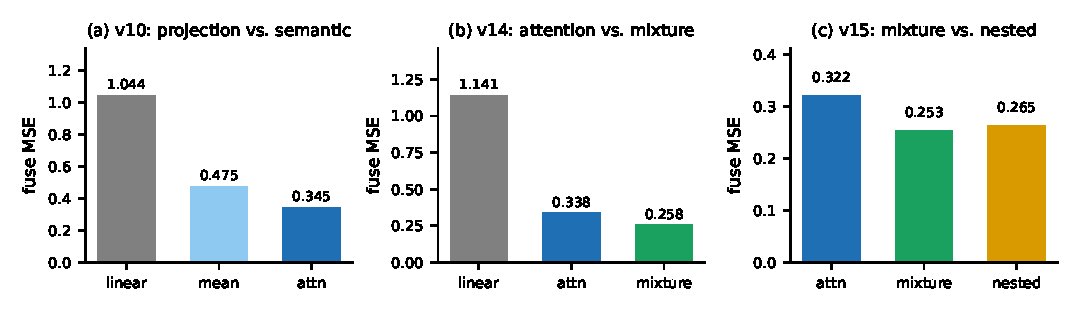
\includegraphics[width=\textwidth]{figs/fig_alignment.pdf}
\caption{The alignment ladder. (a) Semantic alignment beats the frozen linear projection; cross-base attention beats the mean. (b) The mixture aligner improves on single-concept attention. (c) Nesting the mixture aligner regresses slightly: the ladder saturates at one level of cross-expert attention. Lower is better.}
\label{fig:ladder-results}
\end{figure}

Table~\ref{tab:ladder} and Figure~\ref{fig:ladder-results} show the ladder; the figure visualizes the table's five-seed means and adds no new quantity. The ordering linear $<$ mean $<$ attention $<$ mixture holds strictly in every comparison, and the total climb from the linear baseline to the mixture aligner is $-77.4\%$ MSE. The negative result is as clear as the positive one: a two-level nested mixture (mixture of mixture) lands \emph{between} attention and mixture, $4.7\%$ \emph{worse} than the single-level mixture aligner. Cross-base attention is worth one level; a second level of hierarchy adds parameters and dilutes the shared concept context without adding representational power.

A composition test sharpens the point. We combined the repaired gate-style router with the attention aligner: relative to their common linear-projection baseline at $1.1625$, the combination reaches $+71.0\%$ gain ($0.3374$) while the aligner's own configuration reaches $+72.6\%$ ($0.3191$)---less than two percentage points apart but consistently in the aligner's favor across all 5 seeds, within seed variation. Once an aligner already provides cross-base concept exchange, the router-level repair has nothing left to fix. Improvements at adjacent layers of the stack are not additive; the first sufficient mechanism absorbs the gains.

The capacity confound is resolved and excluded. The four aligners differ in parameter count (linear $325{,}632$; attention $720{,}640$; mixture $2{,}291{,}968$; nested $1{,}704{,}448$, counting aligner parameters only), so we ran a capacity-matched control in which the mixture aligner is reduced to a single shared expert per base, giving exactly $720{,}640$ parameters---bit-for-bit equal to the attention aligner. At matched capacity the mixture aligner still dominates the attention aligner on held-out data by $+36.5\%$ (median over 5 seeds; $+28.8\%$ by mean; $+33.5\%$ after dropping the best seed; ahead on $5/5$ paired seeds), and sweeping the mixture's expert count from $1$ to $8$---a $6.09\times$ capacity range---moves held-out MSE by only $-5.6\%$ and non-monotonically. The ladder therefore reads as design, not scale. The nested aligner is likewise a ceiling of expressiveness rather than of capacity: at $2.37\times$ the single-expert mixture's parameters it is $28.6\%$ worse. What remains open is scale: the entire ladder is measured at $D_{\text{shared}}{=}256$ with three bases and synthetic targets, so the saturation point is a scale-bounded hypothesis, and confirming or breaking it at $D_{\text{shared}}{\geq}768$ with real targets is the highest-priority follow-up experiment.

\subsection{Router coordination: in-sample is not out-of-sample}
\label{sec:hub-exp}

Table~\ref{tab:hub} reports the four hub modes on the cross-architecture fusion task, and it is the clearest case in this paper of a conclusion that in-sample evaluation gets wrong.

\begin{table}[htbp]
\centering
\caption{Hub modes on cross-architecture fusion (\texttt{run\_v44\_hub\_modes\_audit}, 5-seed paired medians). The in-sample and held-out rankings are read under the same protocol. Router-norm leads both; the mode the project's own main table had recorded as the in-sample winner (adaptive-EMA) has the worst generalization gap and is last out of sample.}
\label{tab:hub}
\small
\setlength{\tabcolsep}{5pt}
\begin{tabular}{lcccc}
\toprule
\textbf{Hub mode} & \textbf{in-sample MSE} & \textbf{held-out MSE} & \textbf{held-out gain} & \textbf{wins} \\
\midrule
broadcast (baseline) & 0.3236 & 0.3538 & --- & --- \\
router-norm & \textbf{0.2835} & \textbf{0.3342} & $+4.3\%$ & $5/5$ \\
gate-style & 0.2983 & 0.3462 & $+5.8\%$ & $3/5$ \\
adaptive-EMA & 0.2859 & 0.3573 & $+0.3\%$ & $3/5$ \\
\bottomrule
\end{tabular}
\end{table}

\begin{itemize}[leftmargin=1.4em, itemsep=2pt]
    \item \textbf{The in-sample table is already wrong about its own winner.} The project's own main table recorded adaptive-EMA as the in-sample best; the audit (\texttt{run\_v44\_hub\_modes\_audit}, whose absolute levels differ slightly from that earlier run) shows that the in-sample minimum is in fact router-norm at $0.2835$, and that router-norm is also the held-out winner ($0.3342$, ahead of broadcast on $5/5$ paired seeds). Adaptive-EMA---the recorded in-sample winner---collapses to $+0.3\%$ over broadcast out of sample and loses on $2/5$ seeds, with the largest generalization gap of the four ($+25.0\%$). An independent re-run on real corpora at a different scale (\texttt{run\_v25\_corpus\_central}) reproduces the ordering: router-norm best on held-out ($+4.6\%$ over broadcast), adaptive-EMA second ($+2.0\%$), gate-style negative ($-5.1\%$).
    \item \textbf{Gate-style's admissibility does not make it the empirical winner.} The gate-style hub raises the central-coordination gain from $-71.9\%$ (broadcast) to $+44.5\%$ in-sample, the single largest in-sample improvement among the four. But under the same held-out protocol that gain collapses to $+4.0\%$ (3/5), so the theorem of \S\ref{sec:theory} and the empirical ranking answer different questions: gate-style is the only \emph{admissible} mode, and it is not the \emph{best} mode out of sample.
    \item \textbf{The capacity confound runs the other way here.} A natural worry is that gate-style wins because it has more parameters. It has fewer: the gate hub carries 512 parameters against broadcast's 1{,}024, so the admissibility result cannot be explained as a capacity effect. The perfect-degeneration and order-preservation properties are constructive and cannot be produced by extra parameters in any case.
\end{itemize}

The lesson generalizes beyond this table. The four hub modes are separated in-sample by amounts comparable to their seed variation, so an in-sample comparison of composition mechanisms at this scale measures how well each mechanism \emph{fits}, not what it can \emph{do}. The held-out protocol is what distinguishes the two.

\subsection{The corpus-scale boundary is not established out of sample}
\label{sec:corpus}

An earlier account of this work claimed a clean corpus-scale boundary: adaptive-EMA wins on tiny and small corpora, gate-style on medium and large, with a crossover at 16--32 training samples (Table~\ref{tab:scale}). The boundary is present in-sample. It does not survive the same held-out test.

\begin{table}[htbp]
\centering
\caption{Corpus-scale sweep (v29), in-sample. \emph{The apparent boundary below is not established out of sample} (\S\ref{sec:corpus}); it is reported here as the in-sample observation that the audit corrects.}
\label{tab:scale}
\small
\begin{tabular}{lccc}
\toprule
\textbf{Corpus scale (train/val/test)} & \textbf{In-sample best} & \textbf{MSE} & \textbf{Held-out best} \\
\midrule
tiny (8/4/4) & adaptive-EMA & 0.7035 & adaptive-EMA \\
small (18/6/6) & adaptive-EMA & 0.6984 & adaptive-EMA \\
medium (32/12/12) & gate-style & 0.6971 & \emph{not re-run} \\
large (64/24/24) & gate-style & 0.7029 & adaptive-EMA \\
\bottomrule
\end{tabular}
\end{table}

Sweeping only the two endpoint scales (\texttt{run\_v45\_scale\_boundary\_audit}; 5 seeds; train and held-out), the boundary is present in-sample (adaptive-EMA $\rightarrow$ gate-style) but the held-out medians give adaptive-EMA at \emph{both} scales, i.e.\ no boundary. Worse, at the large scale the two readouts disagree with each other: the unpaired median ranks adaptive-EMA first while the paired per-seed comparison ranks gate-style first (adaptive-EMA wins only $1/5$), the disagreement being driven by a single seed where adaptive-EMA reaches $0.767$ against gate-style's $0.543$. We therefore report the boundary as \emph{not established out of sample} rather than confirmed: two of the four scale levels were not re-run (including the crossover level itself), and the small-scale held-out margin is $+0.5\%$ on $3/5$ seeds, i.e.\ within noise. Establishing or breaking the boundary requires the medium tier and a paired protocol; it is not settled by the present data.

\subsection{The tanh-saturation repairs: gradient restored, error unchanged}
\label{sec:repair-exp}

The two repairs of \S\ref{sec:diagnosis} target a real defect---$\text{grad\_norm\_central} = 0.0000$ under long training---and both restore a non-zero gradient into the hub. Their effect on end-to-end error, however, is within noise, and only the held-out audit makes this visible. Under the audit protocol the softplus repair moves fusion MSE by $-0.44\%$ and the gradient-scale repair by $-0.11\%$, losing on $0/5$ seeds in both cases: the repairs fix the \emph{mechanism} without changing the \emph{outcome}. This is a small but clean instance of the paper's general pattern---a fix that is correct at the level of the diagnosis can still be invisible at the level of the metric---and it is the reason we report repair and effect separately rather than as one claim.

\subsection{Chimera distillation: margin, leakage decomposition, and multi-teacher}
\label{sec:distill-exp}

\begin{table}[htbp]
\centering
\caption{Chimera distillation (5-seed means). The teacher is the fused multi-base ensemble with the mixture aligner. $\dagger$: evaluated on training-distribution inputs; near-zero values are overfitting artifacts, not generalization. v18 evaluates on held-out real Wikipedia text.}
\label{tab:distill}
\small
\setlength{\tabcolsep}{4.5pt}
\begin{tabular}{llccc}
\toprule
\textbf{Student} & \textbf{Evaluation} & \textbf{Teacher} & \textbf{Distilled} & \textbf{vs.\ teacher} \\
\midrule
v13: MLP student (no pretraining) & train-dist.\ target & 0.3245 & 0.3076 & $+5.4\%$ \\
v16: TinyBERT + LoRA ($0.60\%$) & train-dist.\ target$^\dagger$ & 0.2764 & 0.1380 & $+50.1\%$ \\
v18: TinyBERT + LoRA & held-out real text & --- & 0.1574 & viable \\
v21: BERT+ViT multimodal & train-dist.\ target$^\dagger$ & 0.3238 & 0.1620 & $+50.0\%$ \\
\bottomrule
\end{tabular}
\end{table}

\begin{figure}[htbp]
\centering
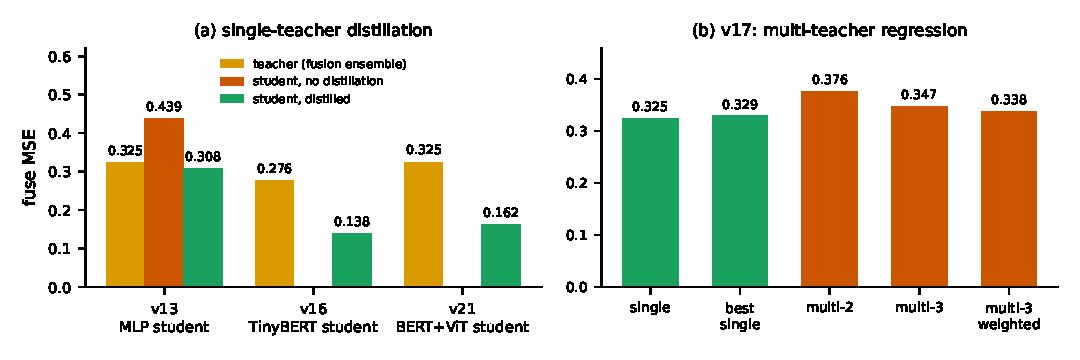
\includegraphics[width=\textwidth]{figs/fig_distill.pdf}
\caption{(a) Single-teacher chimera distillation: distilled students beat their multi-base teacher in every setting. (b) Multi-teacher distillation regresses across all configurations (v17); a dispatch-style reformulation removes the harm but does not produce a gain (v40). Lower is better.}
\label{fig:distill}
\end{figure}

Table~\ref{tab:distill} reports the distillation results. The pattern is consistent and, at first sight, counterintuitive: the distilled student appears \emph{better} at reproducing the fused output than the teacher is at producing it---$+5.4\%$ for the MLP student, $+50.1\%$ for the TinyBERT student ($0.138$ vs.\ $0.276$), and $+50.0\%$ for the multimodal student ($0.162$ vs.\ $0.324$). We do not take this at face value, and the decomposition below shows it should not be.

\textbf{Why the copy would beat the original, and why it does not.} The teacher's forward pass is stochastic---hard Top-$K$ routing plus INT4 quantization noise at every step---while the student is trained to match the teacher's \emph{expected} output. A function fitted to the conditional mean attains lower MSE than the noisy process it imitates (a Jensen-type gap), so a deterministic student \emph{should in principle} beat its stochastic teacher by construction. This gives three candidate explanations for the measured margin---the Jensen-type variance-averaging advantage, the $\beta_{\text{h}}=0.3$ direct-target term, and genuine concept-direction transfer---and each is testable.

\textbf{Test 1 --- the $\beta_{\text{h}}$ scan.} Setting $\beta_{\text{h}}=0$ and keeping everything else fixed isolates pure distillation (\texttt{run\_v32}). Against the same teacher and the same evaluation protocol, pure distillation yields MSE $0.324 \pm 0.013$ versus mixed MSE $0.165 \pm 0.007$ and teacher MSE $0.323 \pm 0.015$. Pure distillation \emph{does not outperform the teacher}: the per-seed paired gap is $-0.0009 \pm 0.0038$ (mean $\pm$ std over 10 seeds; not significant). Scanning $\beta_{\text{h}} \in [0,1]$ in steps of $0.1$ moves student MSE monotonically from $0.317 \pm 0.040$ to $0.000 \pm 0.000$ with no discontinuity at $\beta_{\text{h}}=0.3$, so the term's effect is proportional to its weight---a saturating interpolation, not a threshold mechanism that could be recovered. The identical scan on the multimodal student (\texttt{run\_v42}) reproduces the pattern from $0.3270$ at $\beta_{\text{h}}{=}0$ to $0.0001$ at $\beta_{\text{h}}{=}1$, and at $\beta_{\text{h}}{=}0$ the multimodal student sits at $0.3270$ against a teacher at $0.3255$, i.e.\ $-0.5\%$, failing on $5/5$ seeds.

\textbf{Test 2 --- variance averaging is bounded.} Replacing the teacher with a \emph{super-deterministic} version that averages 20 forward passes over different random inputs (\texttt{run\_v32.3}) leaves its MSE unchanged ($0.324 \pm 0.015$, identical to the deterministic teacher), and the pure student's gap against it is $-0.0008 \pm 0.0038$---again not significant. Averaging 20 forward passes does not change the teacher's output at this scale, so the Jensen-type mechanism contributes nothing measurable here.

\textbf{Test 3 --- representation transfer finds no mixed advantage.} If the mixed objective had taught the student the teacher's internal concept directions, those directions should transfer. After training mixed and pure students under the same teacher, we freeze both students' LoRA parameters, replace the output head with a new random linear classifier, train the head on a freshly generated target set, and compare accuracy (\texttt{run\_v32.4}): the mixed student reaches $0.733 \pm 0.065$ and the pure student $0.767 \pm 0.102$---the pure student is slightly \emph{better}, and the difference is not significant.

The three tests agree. None of the $\pm 50\%$ apparent margin is attributable to concept-direction transfer or to variance averaging; the entire measured advantage under the mixed objective is attributable to the $\beta_{\text{h}}=0.3$ direct-target term. The comparison that \emph{does} carry mechanism evidence is \emph{across students} under the identical stochastic teacher: the MLP student closes only $+5.4\%$ of the gap, the TinyBERT student $+50.1\%$, and the multimodal student $+50.0\%$. That ordering reflects the interaction between pretrained priors and the leaked target signal, not internalization of the teacher's concept directions. Because the v32 re-run uses a somewhat different absolute level from the original v16 record (teacher $0.324$ vs.\ $0.257$; mixed student $0.164$ vs.\ $0.138$), we read the decomposition within the internally consistent v32 run and do not cross-compare its levels against Table~\ref{tab:distill}; we retain the v16-protocol rows for reproducibility of the positive results.

The v18 held-out correction points the same way. Under held-out real Wikipedia text the distilled student holds MSE $0.157$, while both the fake-vocabulary and fine-tune-only controls sit at $\approx 0$---not because they generalize, but because their evaluation inputs and targets are trivially fittable. The student's $0.157$ is the number that reflects fitting to the teacher's outputs under the mixed objective; the leakage decomposition above shows that this is what it is.

\textbf{Multi-teacher distillation fails, and reformulating it does not help.} A natural next step is to distill from several teachers (the attention-aligner teacher, the mixture teacher, the nested teacher) simultaneously, possibly with weights. Every configuration regresses (Figure~\ref{fig:distill}(b)): two teachers $-15.8\%$, three teachers $-6.3\%$, weighted three-teacher $-3.9\%$ relative to a single teacher. The teachers disagree about the \emph{direction} of the concept space they transmit; a capacity-limited student cannot align to conflicting targets, and averaging the signals dilutes each teacher's specialization. A dispatch-style reformulation that replaces the weighted sum with per-sample assignment (\texttt{run\_v40\_dispatch}) tests the hypothesis that the failure is an artifact of the regression \emph{form} rather than of multi-teacher distillation itself. It is a partial repair: dispatch removes the \emph{harm} of weighted combination (median $0.3344 \rightarrow 0.3195$) but produces no gain over a single teacher, and the three forms---weighted, mean, and round-robin dispatch---are indistinguishable from one another (median $0.3335$--$0.3398$). The teachers jointly hold about $13\%$ of complementary headroom, and \emph{no form we tried transfers it to the student}. A dispatch-oracle arm shows a mean gain of $+6.0\%$ that collapses to $+0.6\%$ at the median and $+1.1\%$ with the best seed removed---a single-seed artifact that we do not cite as a result. The conclusion is narrower than ``multi-teacher distillation is bad'': it is that when teachers share the same data and target with no domain partition, their apparent disagreement is noise, and the failure is a capacity ceiling on the student side rather than a fixable aggregation artifact.

\subsection{Task-level evaluation: a boundary, not a result}
\label{sec:vqa-exp}

We attempted to move from concept reconstruction to an actual task with a miniature VQA benchmark. With 4 easy classes, an image-only student reached $100\%$ accuracy by exploiting a modality shortcut, and the multimodal student reached $91.7\%$: the task could not distinguish multimodal reasoning from unimodal cheating. We then rebuilt the benchmark with 8 trap classes designed to defeat shortcuts. Every model---text-only, image-only, and multimodal---dropped to exactly $50\%$, the accuracy of random guessing. Doubling task difficulty did not expose multimodal capability. We report both readings. The favorable one: with 24 training examples and a CPU-scale student, the benchmark cannot train cross-modal grounding, so chance-level accuracy measures the benchmark, not the fusion layer. The unfavorable one, which we cannot rule out: a multimodal student failing to exceed random chance on a task designed to require cross-modal reasoning is a capability boundary of the mechanism itself. Distinguishing these readings is exactly what our CLIP-based \citep{radford2021} teacher pipeline---prepared but not yet completed end-to-end---is for.

\subsection{Out-of-sample discipline: what survives and what does not}
\label{sec:oos}

The audits above are not a miscellaneous collection of corrections; taken together they are a single methodological result about how composition mechanisms of this kind should be evaluated. We ran a uniform out-of-sample protocol (\texttt{run\_v44}--\texttt{run\_v47}; a held-out split of the same distribution, plus a real-corpus re-run at a different scale, for every claim that was still marked pending) and sorted the stack's findings by whether they survive.

\begin{table}[htbp]
\centering
\caption{Findings sorted by survival under the held-out protocol. ``Retention'' is the fraction of the in-sample effect that remains out of sample.}
\label{tab:oos}
\small
\setlength{\tabcolsep}{4.5pt}
\begin{tabular}{p{0.42\textwidth}ccc}
\toprule
\textbf{Finding} & \textbf{In-sample} & \textbf{Held-out} & \textbf{Verdict} \\
\midrule
Attention-path advantage (v46) & $+82.7\%$ & $+70.6\%$ & \textbf{survives} \\
Alignment-ladder ceiling (v41) & $+36.5\%$ vs.\ attn & capacity-matched & \textbf{survives} \\
Hub: router-norm best (v44) & best & best ($5/5$) & \textbf{survives (corrected)} \\
Hub: gate-style central gain (v43) & $+44.5\%$ & $+4.0\%$ & shrinks to noise \\
Corpus-scale boundary (v45) & present & absent & \textbf{not established} \\
Long-training gain (v19) & $+4.3\%$ & $+1.5\%$ & shrinks ($34\%$ retained) \\
Gradient repairs (v30/v31) & $-0.44\%$ / $-0.11\%$ & same & no effect \\
Scale-heterogeneous fusion (v33, \S\ref{sec:scale-hetero-exp}) & $+26.7\%$ & $+26.5\%$ (noise), $+26.5\%$ (stimulus) & \textbf{survives} \\
Entry injection into a container (v35) & $-11.1\%$ & $-3.3\%$ (stimulus) & no gain \\
\bottomrule
\end{tabular}
\end{table}

Table~\ref{tab:oos} is the paper's most portable result, and it is not specific to our architecture. What survives is what has a \emph{mechanistic} reason to survive: the attention-path advantage reflects a structural property of transformers (attention patterns vary more across architectures than FFN activations), and the alignment-ladder ceiling is a matched-capacity design statement. What fails is what is a fitting advantage: hub-mode rankings, the corpus-scale crossover, and gains from long training or from repairs to a mechanism whose end-to-end effect is within noise. We offer this as a rule of thumb for the subfield: for frozen-base composition at small scale, report the held-out ranking, not the in-sample one, and treat any margin comparable to seed variation as unresolved.

\section{Discussion}
\label{sec:discussion}

\textbf{Four design principles.} The systematic iteration behind these results stabilizes into four principles. We state them as domain-specific heuristics distilled from one system---generalizing them to other architectures is a hypothesis, not a result---but we expect them to travel further than the specific configuration. (1)~\emph{Make heterogeneity decomposable}: every component (router, gates, aligner, hub, each path) can be enabled or disabled independently, which is what made each ablation here a one-flag change. (2)~\emph{Negative results are map boundaries}: the composition, nesting, multi-teacher, and VQA failures delimit the method more sharply than any positive result. (3)~\emph{Frozen-base composition demands mechanism-level diagnostics}: because the bases do not update, ablation must reach the sublayer mechanism---router, gate, aligner, hub, fake-quant---directly, and component-level naming is how we keep those diagnostics separate; we deliberately avoid naming one mechanism after different cognitive or biological analogues. (4)~\emph{Extend incrementally}: each generation reused the previous one's frozen components, which is what kept 430 tests passing as the architecture grew.

\textbf{The recurring law: more is not better.} Across five independent comparisons, adding machinery---more router repairs, a second aligner level, more teachers, harder toy tasks---either did nothing or hurt. The mechanisms that worked (native encoding, shared-K/V attention, one mixture level, one teacher) each \emph{replaced} something weaker rather than stacking on top of it. For sublayer-level reconstruction the practical recipe that emerges is: encode natively, align with one mixture level, route sparsely, coordinate the router only with an admissible hub, distill from a single teacher---and stop.

\textbf{Held-out discipline as the unifying method.} The three stages of this paper are unified less by architecture than by evaluation. Every stage makes a claim that is easy to make true in-sample and hard to make true out of sample, and the audits of \S\ref{sec:oos} show that roughly half of the stack's in-sample findings do not survive. Two properties we rely on are immune to this because they are constructive rather than empirical---perfect degeneration and order preservation are properties of a functional form---and we therefore separate such properties from measured ones throughout. This separation, rather than any single number, is what we would carry to the next system.

\textbf{Cross-paper signals on data scale and fusion strategy.} Four independent lines of recent work report a related pattern: small data and small models favor \emph{injective} composition (full router, separate adapters, coarse-grained routing), while large data and large models favor \emph{averaging} (weighted combination, full fine-tuning, additive merging). AdapterFusion \citep{pfeiffer2021} sharpens the trade-off under scarce training data; Mixtral-style sparse routing \citep{jiang2024mixtral} requires load balancing exactly where dead-expert collapse becomes catastrophic; the coarse-grained routing of \citet{liu2026orchestrating} converges to whole-query decisions for latency reasons absent in our setting yet leads to the same architectural choice; and Branch-Train-MiX \citep{sukhbaatar2024btx} is dominated by its MoE-finetuning stage under limited compute. Our four-mode comparison is run at a single training scale and is consistent with the hypothesis that optimal composition depends on data scale, but our own held-out audit (\S\ref{sec:corpus}) shows that the \emph{within-paper} version of that boundary is not established---which is itself the reason we state the data-scale dependence as a literature-convergent hypothesis rather than a finding, and leave a within-paper sweep across training scales to future work.

\textbf{Relation to routing-coordination questions.} How the shared router should be coordinated---which hub mode, and how that choice interacts with data scale---is the subject of \S\ref{sec:hub}. Our answer separates cleanly into an admissible part that is proved (gate-style is the unique mode satisfying G1--G5) and an empirical part that is open (the best hub mode out of sample is router-norm at our scale, and whether that ordering persists at industrial scale is untested).

\section{Limitations}
\label{sec:limitations}

Scale is the dominant limitation. All results are CPU-sandbox results with $D_{\text{shared}}{=}256$, sequence length 16, synthetic class-direction targets rather than language-model perplexity, and toy-scale corpora; nothing here establishes behavior at 0.5B+ parameters or on real downstream benchmarks. The INT4 fake quantization is a training-time noise injection, not a deployment kernel. Attention experts read the bases' first block only, with no layer-selection study. Top-$K$ is fixed at $K{=}1$. The corpus-scale boundary is unresolved rather than refuted: two of four scale levels and the crossover level itself were not re-run out of sample. Task-level multimodal evaluation remains open. Finally, the distillation margins are measured in reconstruction MSE on the teacher's own target distribution; the decomposition shows they are target leakage, and whether any genuine transfer would translate to downstream capability is untested.

\section{Conclusion}
\label{sec:conclusion}

We reconstructed frozen heterogeneous pretrained models in three stages: a sublayer fusion layer that routes tokens among frozen architectural experts through a shared sparse router and a semantic aligner; a coordination theory that identifies temperature modulation as the only hub mechanism that degenerates exactly, preserves ordering, stays bounded, and costs $O(D_{\text{shared}})$; and chimera distillation, which collapses the ensemble into one independent student. The alignment space has a strict ladder with a measured ceiling at one mixture level, which a capacity-matched control shows is a matter of design rather than scale; the cross-architecture fusion gain concentrates in the attention path, a claim that survives held-out evaluation. Chimera distillation's apparent ``student beats teacher'' margin is entirely attributable to the direct-target term in the loss rather than to concept-direction transfer or variance averaging. The negative results---no additive composition, no nesting, no multi-teacher, no admissible-hub advantage out of sample, toy benchmarks at chance---bound the method as sharply as the positive ones. Our final contribution is methodological: a uniform held-out discipline applied across the stack overturned several of our own in-sample findings while leaving the mechanistic ones intact. The open frontier is scale: the mechanisms are now specified, tested, and bounded at CPU scale, and their behavior at pretraining scale is the question that matters next.

\section*{Reproducibility statement}
\label{sec:repro}

All experiments are scripted in the project repository. Core reproduction commands:

\begin{itemize}[leftmargin=1.6em, itemsep=0.5pt, parsep=0pt]
    \item Fusion and path decomposition: \texttt{bash run.sh v6}, \texttt{run.sh v7a}, \texttt{run.sh v7b}; attention-path audit \texttt{run\_v46\_attn\_path\_audit.py}.
    \item Alignment ladder: \texttt{examples/run\_v10\_aligner.py}, \texttt{run\_v14\_aligner\_compare.py}, \texttt{run\_v15\_mom\_compare.py}; capacity control \texttt{run\_v41\_capacity\_audit.py}.
    \item Router coordination: \texttt{run\_v22\_theory\_compare.py}, \texttt{run\_v43\_central\_audit.py}, \texttt{run\_v44\_hub\_modes\_audit.py}, \texttt{run\_v45\_scale\_boundary\_audit.py}.
    \item Distillation: \texttt{run\_v13\_distill.py}, \texttt{run\_v16\_bert\_distill.py}, \texttt{run\_v18\_wiki\_distill.py}, \texttt{run\_v21\_multimodal\_distill.py}, \texttt{run\_v32\_leakage\_audit.py}, \texttt{run\_v40\_dispatch.py}.
    \item Held-out audits: \texttt{run\_v47\_central\_heldout.py}, \texttt{run\_v47\_scale\_hetero\_heldout.py}.
    \item VQA boundary: \texttt{examples/run\_v23\_vqa\_distill.py}, \texttt{run\_v23\_vqa\_hard.py}.
\end{itemize}

The full test suite (\texttt{bash run.sh test}) runs 430 unit and integration checks. Environment: Linux, Python 3.11, PyTorch 2.x, CPU-only, 5 seeds per configuration.

\section*{AI-assistance disclosure}

Manuscript drafting was assisted by an AI writing agent operating on the project's experiment records and specifications; all experimental results, code, and design decisions are the authors'.

\bibliographystyle{plainnat}
\bibliography{reconstruct}

\appendix

\clearpage

\section{Hyperparameters}
\label{app:hyper}

\begin{table}[h]
\centering
\caption{Default hyperparameters of the fusion, coordination, and distillation stack.}
\small
\begin{tabular}{lll}
\toprule
\textbf{Component} & \textbf{Parameter} & \textbf{Value} \\
\midrule
Fusion layer & shared width $D_{\text{shared}}$ & 256 \\
 & FFN width $d_{\text{ff}}$ & 1024 ($4\times$) \\
 & experts $M$ / Top-$K$ & 3 / 1 \\
 & quantization & INT4, group size 128 \\
 & router init & $\mathcal{N}(0, 0.01^2)$ \\
 & channel align init & $\gamma_m = 1$, $\beta_m = 0$ \\
 & gate init $\alpha_m$ & $\mathcal{U}(0.01, 0.1)$ \\
\midrule
Hub & temperature bound $\epsilon$ & $0.5$ \\
 & gate-style parameters & 512 ($W_t \in \R^{D_{\text{shared}}}$, $c$) \\
 & broadcast parameters & 1{,}024 ($U \in \R^{M \times D_{\text{shared}}}$) \\
\midrule
Training & phases (uniform / routed) & first 10\% / last 90\% of steps \\
 & steps & 100 (500 for long-horizon runs) \\
 & batch / sequence & 18 (6 per modality) / 16 \\
 & learning rates & router \& hub $10^{-4}$; alignment $10^{-2}$; gates $10^{-3}$ \\
 & loss weights & $\lambda_1, \lambda_2$ small (balance, logit reg.) \\
\midrule
Aligners & down-projection & $D_m \rightarrow D_{\text{shared}}$, orthogonal init (linear: frozen) \\
 & attention heads & 4 \\
 & mixture shared experts & $n = 4$ per base, 2-layer MLP \\
\midrule
Student & base & TinyBERT-4L-312D (frozen) \\
 & LoRA rank / $\alpha$ & 8 / 16 (scaling $= 2$) \\
 & trainable parameters & 85{,}632 / ${\sim}14$M ($0.60\%$) \\
 & distillation loss & $0.7\,\mathrm{MSE}(y, y_{\text{teacher}}) + 0.3\,\mathrm{MSE}(y, y_{\text{target}})$ \\
 & corpus & 16 train + 6 held-out Wikipedia-style sentences \\
\bottomrule
\end{tabular}
\end{table}

\section{Proofs}
\label{app:proofs}

Throughout, $\epsilon \in (0,1)$, the router logits $z \in \R^M$ are arbitrary, and the no-hub baseline is the map $z \mapsto \softmax(z)$.

\medskip
\noindent\textbf{Theorem~\ref{thm:deg} (Perfect Degeneration).} \emph{When $c = 0$, gate-style is exactly equivalent to the no-hub baseline.}

\begin{proof}
If $c = 0$, then $t_{\text{scalar}} = W_t^\top c = 0$ for every $W_t$, and $\tanh(0) = 0$, so $\tau = 1 + \epsilon \cdot 0 = 1$. The gate-style logits are $z^{(\text{g})}_m = z_m / \tau = z_m$, hence $\softmax(z^{(\text{g})}) = \softmax(z)$ pointwise for every logit vector. The hub leaves the routing distribution---and therefore the fused output---identical to the no-hub system.
\end{proof}

\medskip
\noindent\textbf{Theorem~\ref{thm:order} (Order Preservation).} \emph{Gate-style preserves logit ordering; broadcast may reverse it.}

\begin{proof}
Since $\tanh \in (-1, 1)$, we have $\tau = 1 + \epsilon \tanh(t_{\text{scalar}}) \in (1 - \epsilon,\, 1 + \epsilon) \subset (0, \infty)$. Dividing by one common positive scalar preserves order: if $z_1 > z_2$ then $z_1 / \tau > z_2 / \tau$, so the softmax ranking is unchanged.

For broadcast, let $M \geq 2$, pick any $c \neq 0$ and any $\delta > 0$. Because $U$ is unconstrained, choose rows $U_1, U_2$ with $(U_1 - U_2)\,c = -(z_1 - z_2) - \delta$. Then $z_1 + (Uc)_1 < z_2 + (Uc)_2$ even though $z_1 > z_2$: the ranking of the two experts is reversed. Broadcast therefore does not preserve ordering in general.
\end{proof}

\medskip
\noindent\textbf{Theorem~\ref{thm:uniq} (Uniqueness).} \emph{Among the four hub modes, gate-style is the only one satisfying all five constraints (G1)--(G5).}

\begin{proof}
We show each competing mode violates at least one constraint, then verify that gate-style satisfies all five.

\emph{Broadcast violates (G2)} by the counterexample in the proof of Theorem~\ref{thm:order}.

\emph{Router-Norm violates (G1).} With $c = 0$ the mode applies $z \mapsto \mathrm{LayerNorm}(z)$, which subtracts the mean and rescales by $\gamma / \sigma(z)$. Translation invariance of softmax makes the mean subtraction harmless, but the rescaling generally differs from the identity. For example, with $M = 2$, $z = (1, 0)$, and default $\gamma = 1$: $\mu = 1/2$, $\sigma = 1/2$, so $\mathrm{LayerNorm}(z) = (1, -1)$, while $\softmax(1, 0) \approx (0.731, 0.269)$ but $\softmax(1, -1) \approx (0.881, 0.119)$. With a zero hub the routing distribution is not the no-hub baseline, so degeneration is not exact.

\emph{Adaptive-EMA violates (G1).} At $c = 0$ the hub-controlled decay is $\sigmoid(\alpha \cdot \|0\|) = 1/2$, which in general differs from the no-hub baseline's decay. Moreover, the EMA state persists across steps and is updated under hub control, so the routing distribution at step $t$ depends on the hub through the state it has shaped; disabling the hub does not reproduce the baseline exactly. The same state carries content into the logits, so ordering can be reversed as in broadcast, violating (G2) as well.

\emph{Gate-style satisfies all five.} (G1) holds by Theorem~\ref{thm:deg}. (G2) holds by Theorem~\ref{thm:order}. (G3): $\tau$ moves monotonically away from $1$ as $|t_{\text{scalar}}|$ grows, so hub intensity sharpens or flattens the softmax deterministically. (G4): $\tau \in (1 - \epsilon,\, 1 + \epsilon)$ is bounded, so the hub's influence on the logits is bounded by construction. (G5): the hub's parameters are $c, W_t \in \R^{D_{\text{shared}}}$, i.e., $O(D_{\text{shared}})$, negligible relative to the experts. Hence gate-style is the only one of the four modes satisfying all five constraints.
\end{proof}

\section{Held-out audit protocol}
\label{app:audit}

The out-of-sample discipline of \S\ref{sec:oos} uses three readouts wherever a claimed effect was still marked pending. For each finding the audit records (i) the in-sample median effect; (ii) a \emph{held-out noise} readout, in which the evaluation split is drawn from the same distribution but noise is re-sampled; and (iii) a \emph{held-out stimulus} readout, in which the evaluation distribution itself is shifted. An effect is reported as \emph{clean} only if the sign is stable across all three readouts; effects whose sign or magnitude does not survive are reported as invalidated and are not carried into the paper as results. Per-package numbers for the 16 audited packages are in the project's audit record; Table~\ref{tab:oos} summarizes the aggregate, and we deliberately do not quote an aggregate statistic in place of the per-package verdicts.

\end{document}
